\boxde
\Opensolutionfile{ans}[ans/2D1-1-DEON-2]
\begin{ex}%[2D1B1-1]
    Cho hàm số $y=x^3 -2x^2 +x +1$. Mệnh đề nào dưới đây đúng?
    \choice
    {Hàm số đồng biến trên $\left(\dfrac{1}{3};1 \right)$}
    {Hàm số nghịch biến trên $\left(-\infty; \dfrac{1}{3}\right)$}
    {\True Hàm số nghịch biến trên $\left(\dfrac{1}{3}; 1\right)$}
    {Hàm số nghịch biến trên $\left(1; +\infty\right)$}
    \loigiai{
        Tập xác định $\mathscr D = \mathbb{R}$.\\
        $y'=3x^2 -4x +1 $.\\
        Cho $y'=0 \Leftrightarrow \hoac{& x= \dfrac{1}{3} \\&x = 1.}$\\
        Bảng biến thiên
        \begin{center}
            \begin{tikzpicture}[yscale=.8,xscale=1.5,]
                \begin{scope}[shift={(-.5,.5)}]
                    \draw[red]
                    (0,0) rectangle +(8,-5)
                    (0,-1)--+(0:8) (0,-2)--+(0:8) (1,0)--+(-90:5);
                \end{scope}
                \path
                (0,0) node{$x$} % <<< dòng 1
                ++(0:1) node{$-\infty$}
                ++(0:2) node{$\dfrac{1}{3}$}
                ++(0:2) node{$1$}
                ++(0:2) node{$+\infty$}
                (0,-1) node{$y'$} % <<< dòng 2
                ++(0:2) node{$+$}
                ++(0:1) node{$0$}
                ++(0:1) node{$-$}
                ++(0:1) node{$0$}
                ++(0:1) node{$+$}
                (0,-3) node{$y$} % <<< dòng 3
                ++(0:1) ++(-90:1) node (A) {$-\infty$}
                ++(0:2) ++(+90:2) node (B) {$\dfrac{31}{27}$}
                ++(0:2) ++(-90:2) node (C) {$1$}
                ++(0:2) ++(+90:2) node (D) {$+\infty$};
                \draw[-stealth,blue] (A)--(B);
                \draw[-stealth,blue] (B)--(C);
                \draw[-stealth,blue] (C)--(D);
            \end{tikzpicture}
        \end{center}
        Dựa vào bảng biến thiên ta thấy hàm số nghịch biến trên khoảng $\left(\dfrac{1}{3} ; 1\right)$.}
\end{ex}
\begin{ex}%[2D1B1-1]
    Cho hàm số $y= - \dfrac{1}{3} x^3 - x -3 $. Mệnh đề nào dưới đây đúng?
    \choice
    {Hàm số đồng biến trên $(-\infty; 1)$ và trên $(1; +\infty)$}
    {Hàm số đồng biến trên $\mathbb{R}$}
    {\True Hàm số nghịch biến trên $\mathbb{R}$}
    {Hàm số đồng biến trên $(-1;1)$}
    \loigiai{
        Tập xác định $\mathscr D = \mathbb{R}$.\\
        $y'=-x^2 -1<0 $ với mọi $x$.\\
        Suy ra hàm số đã cho nghịch biến trên $\mathbb{R}$.}
\end{ex}
\begin{ex}%[2D1B1-1]
    Cho hàm số $y= \dfrac{1}{3} x^3 - \dfrac{1}{2}x^2 $ nghịch biến trên khoảng có độ dài bằng
    \choice
    {$\dfrac{5}{6}$}
    {$\dfrac{1}{6}$}
    {$\dfrac{\sqrt{37}}{6}$}
    {\True $1$}
    \loigiai{
        Tập xác định $\mathscr D = \mathbb{R}$.\\
        $y'=x^2 -x $.\\
        Cho $y'=0 \Leftrightarrow \hoac{& x= 1\\&x =0 .}$\\
        Bảng biến thiên
        \begin{center}
            \begin{tikzpicture}[yscale=.8,xscale=1.5]
                \begin{scope}[shift={(-.5,.5)}]
                    \draw[red]
                    (0,0) rectangle +(8,-5.1)
                    (0,-1)--+(0:8) (0,-2)--+(0:8) (1,0)--+(-90:5);
                \end{scope}
                \path
                (0,0) node{$x$} % <<< dòng 1
                ++(0:1) node{$-\infty$}
                ++(0:2) node{$0$}
                ++(0:2) node{$1$}
                ++(0:2) node{$+\infty$}
                (0,-1) node{$y'$} % <<< dòng 2
                ++(0:2) node{$+$}
                ++(0:1) node{$0$}
                ++(0:1) node{$-$}
                ++(0:1) node{$0$}
                ++(0:1) node{$+$}
                (0,-3) node{$y$} % <<< dòng 3
                ++(0:1) ++(-90:1) node (A) {$-\infty$}
                ++(0:2) ++(+90:2) node (B) {$0$}
                ++(0:2) ++(-90:2) node (C) {$- \dfrac{1}{6}$}
                ++(0:2) ++(+90:2) node (D) {$+\infty$};
                \draw[-stealth,blue] (A)--(B);
                \draw[-stealth,blue] (B)--(C);
                \draw[-stealth,blue] (C)--(D);
            \end{tikzpicture}
        \end{center}
        Dựa vào bảng biến thiên ta thấy hàm số nghịch biến trên khoảng $( 0; 1)$, có độ dài bằng $1$.}
\end{ex}
\begin{ex}%[2D1B1-1]
    Cho hàm số $y= \dfrac{1}{3} x^4- \dfrac{1}{6}x^2 + 1 $ nghịch biến trên khoảng nào dưới đây?
    \choice
    {$(-\infty; -2) $ và $(0;2)$}
    {$\left(-\dfrac{1}{2} ;0 \right) $ và $\left(-\dfrac{1}{2} ; + \infty \right) $}
    {\True $\left( -\infty; -\dfrac{1}{2} \right) $ và $\left(0; \dfrac{1}{2} \right)$}
    {$ (-2;0) $ và $(2; +\infty)$}
    \loigiai{
        Tập xác định $\mathscr D = \mathbb{R}$.\\
        $y'= \dfrac{4}{3} x^3 - \dfrac{1}{3} x$.\\
        Cho $y'=0 \Leftrightarrow \hoac{& x=0 && \Rightarrow y= 1 \\&x = \pm \dfrac{1}{2} && \Rightarrow y= \dfrac{47}{48}.}$\\
        Bảng biến thiên
        \begin{center}
            \begin{tikzpicture}[yscale=.75,xscale=1]
                \begin{scope}[shift={(-.5,.5)}]
                    \draw[red] (0,0) rectangle +(10,-5.1);
                    \draw (0,-1.2)--+(0:10) (0,-2.2)--+(0:10) (1,0)--+(-90:5);
                \end{scope}
                \path
                (-0.1,0) node{$x$} % <<< dòng 1
                ++(0:1) node{$-\infty$}
                ++(0:2) node{$- \dfrac{1}{2}$}
                ++(0:2) node{$0$}
                ++(0:2) node{$ \dfrac{1}{2}$}
                ++(0:2) node{$+\infty$}
                (0,-1.1) node{$y'$} % <<< dòng 2
                ++(0:2) node{$-$}
                ++(0:1) node{$0$}
                ++(0:1) node{$+$}
                ++(0:1) node{$0$}
                ++(0:1) node{$-$}
                ++(0:1) node{$0$}
                ++(0:1) node{$+$}
                (0,-3) node{$y$} % <<< dòng 3
                ++(0:1) ++(90:1) node (A) {$+\infty$}
                ++(0:2) ++(-90:2) node (B) {$\dfrac{47}{48}$}
                ++(0:2) ++(+90:2) node (C) {$1$}
                ++(0:2) ++(-90:2) node (D) {$\dfrac{47}{48}$}
                ++(0:2) ++(+90:2) node (E) {$+\infty$};
                \draw[-stealth,blue] (A)--(B);
                \draw[-stealth,blue] (B)--(C);
                \draw[-stealth,blue] (C)--(D);
                \draw[-stealth,blue] (D)--(E);
            \end{tikzpicture}
        \end{center}
        Dựa vào bảng biến thiên ta thấy hàm số nghịch biến trên hai khoảng $\left( -\infty; -\dfrac{1}{2} \right) $ và $\left(0; \dfrac{1}{2} \right)$.}
\end{ex}
%Câu 50:
\begin{ex}%[2D1Y1-1]
    Khoảng nghịch biến của hàm số $ y=\dfrac{3-x}{x} $ là khoảng nào dưới đây ?
    \choice
    {$(-\infty ; 3)$ và $ (3 ;+\infty) $}
    {$(-\infty ; 0) \cup(0 ;+\infty)$}
    {$(-\infty ;+\infty)$}
    {\True$(-\infty ; 0)$ và $ (0;+\infty)$ }
    \loigiai{
        Tập xác định: $\mathscr{D} = \mathbb{R}\setminus\{0\}$.\\
        Ta có $ y'=\dfrac{-3}{x^2}<0,\quad \forall x \in \mathscr{D} $. Vậy hàm số nghịch biến trên các khoảng $(-\infty ; 0)$ và $ (0;+\infty)$.
    }
\end{ex}
\begin{ex}%[2D1B1-1]
    Hàm số $f(x)=1-3x^4$ nghịch biến trên khoảng nào sau đây?
    \choice
    {\True $(0;+\infty)$}
    {$(-\infty;0)$}
    {$\left(-\infty ;\dfrac{1}{3}\right)$}
    {$\left(\dfrac{1}{3} ;+\infty\right)$}
    \loigiai{Tập xác định $\mathscr{D}=\mathbb{R}$.\\
        Ta có: $y'=-12x^3$.\\
        Cho $y'=0 \Leftrightarrow -12x^3 = 0 \Leftrightarrow x=0$.\\
        Tại $x=0 \Rightarrow y(0)=1$.\\
        Ta có bảng biến thiên
        \begin{center}
            
\begin{tikzpicture}
                \tkzTabInit[nocadre,lgt=1.2,espcl=2.5,deltacl=0.6]
                {$x$/0.6,$y'$/0.6,$y$/2}
                {$-\infty$,$0$,$+\infty$}
                \tkzTabLine{,+,0,-,}
                \tkzTabVar{-/$-\infty$,+/$1$,-/$-\infty$}
            \end{tikzpicture}
    \end{center}}
\end{ex}
\begin{ex}%[2D1B1-1]
    \immini
    {
        Cho hàm số $y=f(x)$ có đồ thị như hình vẽ. Hàm số đã cho nghịch biến trên khoảng nào sau đây?
        \choice
        {$(-1;1)$}
        {\True $(-1;0)$}
        {$(-\infty;-1)$}
        {$(0;1)$}
    }
    {
        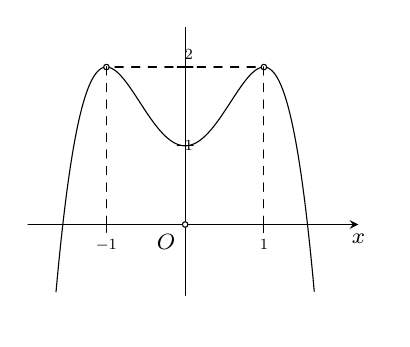
\begin{tikzpicture}[scale=1, line join=round, line cap=round, >=stealth]
            \clip (-2,-1.2) rectangle (2.5,2.5);
            \def\xmin{-1.8}\def\xmax{2}\def\ymin{-0.7}\def\ymax{2.5}
            \draw[->] (\xmin-0.2,0)--(\xmax+0.2,0) node[below] {\footnotesize $x$};
            \draw[->] (0,\ymin-0.2)--(0,\ymax+0.2) node[right] {\footnotesize $y$};
            \draw (0,0) node [below left] {\footnotesize $O$};
            \foreach \x in {,-1,1,}\draw (\x,0.1)--(\x,-0.1) node [below,scale=0.7] {\footnotesize $\x$};
            \foreach \y in {1}\draw (0.1,\y)--(-0.1,\y) node [right=0.2,scale=0.7] {\footnotesize $\y$};
            \foreach \y in {2}\draw (0.1,\y)--(-0.1,\y) node [above right=0.2,scale=0.7] {\footnotesize $\y$};
            \draw[smooth,samples=200,domain=-1.64:1.64] plot (\x,{-1*((\x)^4)+2*((\x)^2)+1});
            \draw[fill=white] (0,0) circle (1pt) (-1,2) circle (1pt) (1,2) circle (1pt) ;
            \draw[dashed] (-1,0)--(-1,2)--(0,2);
            \draw[dashed] (1,0)--(1,2)--(0,2);
        \end{tikzpicture}
    }
    \loigiai{Dựa vào đồ thị hàm số ta thấy đồ thị hàm số giảm trên các khoảng $(-1;0)$ và $(1;+\infty)$.}
\end{ex}
\begin{ex}%[2D1Y1-1]
    Hàm số $ y=-\dfrac{1}{x-4} $ đồng biến trên khoảng nào dưới đây ?
    \choice
    {$(-\infty ; 1)$ và $ (1 ;+\infty) $}
    {\True$(-\infty ; 4)$ và $ (4 ;+\infty) $}
    {$(-\infty ; -4)$ và $ (-4 ;+\infty) $}
    {$(-\infty ; -1)$ và $ (-1 ;+\infty) $}
    \loigiai{
        Tập xác định: $\mathscr{D} = \mathbb{R}\setminus\{4\}$.\\
        Ta có $ y'=\dfrac{1}{(x-4)^2}>0,\quad \forall x \in \mathscr{D} $. Vậy hàm số đồng biến trên $(-\infty ; 4)$ và $ (4 ;+\infty) $.
    }
\end{ex}
%Câu 52:
\begin{ex}%[2D1Y1-1]
    Kết luận nào sau đây về tính đơn điệu của hàm số $ y=\dfrac{2 x+5}{1-x} $ là kết luận \textbf{sai} ?
    \choice
    {Hàm số đồng biến trên $(-\infty ; 1)$ và $ (1 ;+\infty) $}
    {\True Hàm số đồng biến trên $(-\infty ; 1) \cup(1 ;+\infty)$}
    {Hàm số đồng biến trên $(-\infty ; 1)$}
    {Hàm số đồng biến trên $(1 ;+\infty)$}
    \loigiai{
        Tập xác định: $\mathscr{D} = \mathbb{R}\setminus\{1\}$.\\
        Ta có $ y'=\dfrac{7}{(1-x)^2}>0,\quad \forall x \in \mathscr{D} $. Vậy hàm số đồng biến trên $(-\infty ; 1)$ và $ (1 ;+\infty) $.
    }
\end{ex}
\begin{ex}%[2D1B1-1]
    Hàm số nào sau đây nghịch biến trên khoảng $(-\infty;+\infty)$.
    \choice
    {$y=x^{3}-3 x^{2}$}
    {\True $y=-x^{3}+3 x^{2}-3 x+2$}
    {$y=-x^{3}+3 x+1$}
    {$y=x^{3}+2018$}
    \loigiai{Tập xác định $\mathscr{D}=\mathbb{R}$.\\
        Ta có: $y'=-3x^2+6x-3$.\\
        Cho $y'=0 \Leftrightarrow -x^2+3x-1=0 \Leftrightarrow x=1$.\\
        Tại $x=1 \Rightarrow y(1)=1$.\\
        Ta có bảng biến thiên
        \begin{center}
            
\begin{tikzpicture}
                \tkzTabInit[nocadre,lgt=1.2,espcl=2.5,deltacl=0.6]
                {$x$/0.6,$y'$/0.6,$y$/2}
                {$-\infty$,$1$,$+\infty$}
                \tkzTabLine{,-,0,-,}
                \tkzTabVar{+/$+\infty$,R/,-/$-\infty$}
                \tkzTabVal{1}{3}{0.5}{}{$1$}
            \end{tikzpicture}
    \end{center}}
\end{ex}
%Câu 53:
\begin{ex}%[2D1B1-1]
    Hàm số $ y=\dfrac{x^{2}-3 x+5}{x+1} $ nghịch biến trên các khoảng nào sau đây ?
    \choice
    {$(-\infty ;-4)$ và $ (2 ;+\infty) $}
    {$(-4 ; 2)$}
    {\True$(-4 ;-1)$ và $ (-1 ; 2) $}
    {$(-\infty ;-1)$ và $ (-1 ;+\infty) $}
    \loigiai{
        Tập xác định: $\mathscr{D} = \mathbb{R}\setminus\{-1\}$. \\
        Ta có $y'=\dfrac{x^2+2x-8}{(x+1)^2} $. Cho
        $ y'=0 \Leftrightarrow \hoac{& x=-4 \\ & x=2.} $\\
        Bảng biến thiên:
        \begin{center}
            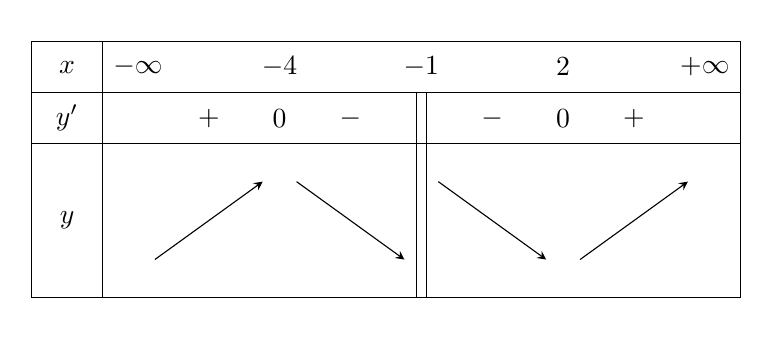
\begin{tikzpicture}[yscale=0.65,xscale=0.9]
                \def\c{9}%số cột
                \def\d{4}%số dòng
                \foreach \x in {0,...,\c}{
                    \foreach \y in {0,...,\d}
                    \path[yscale=-1] (\x,\y) node[gray!0,minimum size=1cm] (\x\y) {\x\y};
                }
                \draw[double,double distance=.12cm,shorten >=-0.83cm, shorten <=-0.18cm](50)--(54);
                \draw[shift={(-0.5,0.5)}]
                (0,0) rectangle (\c+1,-\d-1)
                (0,-1)--(\c+1,-1)
                (0,-2)--(\c+1,-2)
                (1,0)--(1,-\d-1);
                \path
                (00) node {$x$}(10) node {$-\infty$}(30) node {$-4$}(50) node {$-1$}(70) node {$2$}(90) node {$+\infty$}
                (01) node {$y'$}(21) node {$+$}(31) node {$0$}(41) node {$-$}(61) node {$-$}(71) node {$0$}(81) node {$+$}
                (03) node {$y$}
                ;
                \foreach \a/\b in {14/32,32/54,52/74,74/92}
                \draw[->,>=stealth,shorten >=-0.36cm, shorten <=-0.36cm] (\a)--(\b);
            \end{tikzpicture}
        \end{center}
        Dựa vào bảng biến thiên, hàm số nghịch biến trên $(-4 ;-1)$ và $ (-1 ; 2) $.
    }
\end{ex}
%===27
\begin{ex}%[2D1B1-1]
    Hàm số $y=\sqrt{8+2x-x^2}$ đồng biến trên khoảng nào sau đây?
    \choice
    {$(1;+\infty)$}
    {$(1;4)$}
    {$(-\infty;1)$}
    {\True $(-2;1)$}
    \loigiai{
        Tập xác định $\mathscr{D}=[-2;4]$.\\
        $y'=\dfrac{2-2x}{2\sqrt{8+2x-x^2}}$.\\
        \textbf{Cách 1:}\\
        $y'=0\Leftrightarrow x=1$.\\
        Bảng biến thiên
        \begin{center}
            \begin{tikzpicture}[yscale=.8,xscale=1.5,]
                \begin{scope}[shift={(-.5,.5)}]
                    \fill[pattern=north east lines,pattern color=violet](1,-1) rectangle +(1.5,-4) (6.5,-1) rectangle +(1.5,-4);
                    \draw
                    (0,0) rectangle +(8,-5)
                    (0,-1)--+(0:8) (0,-2)--+(0:8) (1,0)--+(-90:5);
                \end{scope}
                \path
                (0,0) node{$x$} % <<< dòng 1
                ++(0:1) node{$-\infty$}
                ++(0:1) node{$-2$}
                ++(0:2) node{$1$}
                ++(0:2) node{$4$}
                ++(0:1) node{$+\infty$}
                (0,-1) node{$y'$} % <<< dòng 2
                ++(0:3) node{$+$}
                ++(0:1) node{$0$}
                ++(0:1) node{$-$}
                (0,-3) node{$y$} % <<< dòng 3
                ++(0:2) ++(-90:1) node (A) {$0$}
                ++(0:2) ++(90:2) node (B) {$3$}
                ++(0:2) ++(-90:2) node (C) {$0$};
                \draw[-stealth] (A)--(B);
                \draw[-stealth] (B)--(C);
                \draw[double] (2,-.5)--(2,-1.5) (6,-.5)--(6,-1.5);
            \end{tikzpicture}
        \end{center}
        \textbf{Cách 2:}\\
        $2-2x>0 \Leftrightarrow x<1$.\\
        $y'>0 \Leftrightarrow -2<x<1$.\\
        Vậy hàm số nghịch biến trên khoảng $(-2;1)$.
    }
\end{ex}
\begin{ex}%[2D1K1-1]
    Cho hàm số $f(x)=x^3+x^2+8x+\cos5x$. Với hai số thực $a<b$, khẳng định nào sau đây đúng?
    \choice
    {$f(a)=f(b)$}
    {$f(a)>f(b)$}
    {\True $f(a)<f(b)$}
    {$f(a)\ge f(b)$}
    \loigiai{
        Do $f'(x)=3x^2+2x+8-5\sin5x =(3x^2+2x+3)+(5-5\sin5x)>0$ nên hàm số luôn đồng biến trên $\mathbb{D}=\mathbb{R}$.\\
        Vì vậy $a<b \Rightarrow f(a)<f(b)$
    }
\end{ex}
%Câu 57
\begin{ex}%[2D1Y1-2]
    \immini
    {
        Cho hàm số $ y=f(x) $ có đồ thị như hình vẽ bên. Hàm số đã cho đồng biến trên khoảng
        \choice
        {\True$(2;3)$}
        {$(0;2)$}
        {$(-2;1)$}
        {$(1;2)$}
    }
    {
        \begin{tikzpicture}[>=stealth,x=1cm,y=1cm,scale=0.5,font=\footnotesize]
            \path
            (0,0) coordinate (O)
            (-0.5,0) coordinate (A)
            %	Các điểm mút cho lệnh controls:
            (-1.5,3.3) coordinate (N)
            (1,1.6) coordinate (M1)
            (2.2,-0.8) coordinate (Q)
            (3.5,3.5) coordinate (M2)
            ;
            %Vẽ đường cong:
            %	\draw[red] (N)--(M1)--(Q)--(M2);
            \draw (N)..controls +(-80:0.5) and +(170:0.5)..(O)..controls +(10:0.5) and +(-170:0.25)..(M1)..controls +(-5:0.5) and +(175:0.5)..(Q)..controls +(5:0.5) and +(-100:0.25)..(M2);
            %Vẽ hệ trục tọa dộ:
            \draw[->] (-2,0)--(0,0) node[below left]{$O$}--(4.3,0) node[below]{$x$};
            \draw[->] (0,-1) --(0,4) node[left]{$y$};
            %	Vẽ nét đứt+node:
            \foreach \p/\n/\r in {N/-2/-90,M1/1/-90,Q/2/90,M2/3/-90}
            \draw[dashed](\p)--($(A)!(\p)!(O)$)node[shift={(\r:3mm)}]{$ \n $} ;
            \path ($(A)!(N)!(O)$)coordinate (A1) ($(A)!(M2)!(O)$)coordinate (B3)($(A)!(Q)!(O)$)coordinate (B2)($(A)!(M1)!(O)$)coordinate (B1);
            \foreach \p in {M1,M2,O,Q,N,A1,B3,B2,B1}
            \fill (\p) circle (1.7pt) ;
        \end{tikzpicture}
    }
    \loigiai{
        Dựa vào đồ thị, hàm số đồng biến trên các khoảng $ (0;1) $ và $ (2;3) $.
    }
\end{ex}
\begin{ex}%[2D1B1-1]
    \immini
    {
        Cho hàm số đa thức $ f(x)$ có đồ thị $y=f'(x)$ như hình vẽ bên dưới. Tìm khẳng định đúng.
        \choice
        {Hàm số $f(x)$ đồng biến trên $(-2 ; 0)$}
        {Hàm số $f(x)$ nghịch biến trên $(0 ;+\infty)$}
        {\True Hàm số $f(x)$ đồng biến trên $(-\infty, 3)$ }
        {Hàm số $f(x)$ nghịch biến trên $(-3 ;-2)$}
    }
    {
        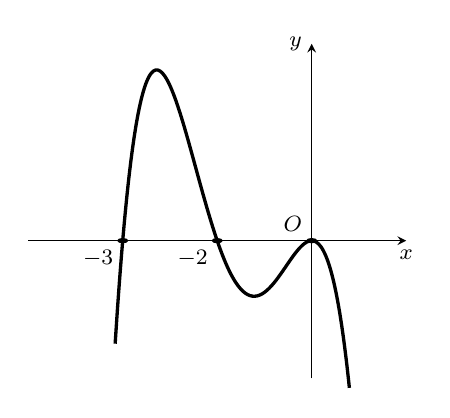
\begin{tikzpicture}[>=stealth,font=\footnotesize, xscale=1.2, yscale=0.5]
            \draw[->] (-3,0) -- (1,0) node[below] {$x$};
            \draw[->] (0,-3.5) -- (0,5) node[left] {$y$};
            \filldraw (0,0) node[above left=-0.1] {$O$} circle (1.5pt);
            %\draw[smooth,samples=100,domain=-2.43:0.43] plot(\x,{-5*(\x+1)^4+10*(\x+1)^2-2}) node[right] {\tiny $y=f(x+1)$};
            \draw[line width=1.2pt, smooth,samples=100,domain=-2.08:0.4] plot(\x,{-7*(\x)^2*(\x+1)*(\x+2)});
            \filldraw (-2,0) node[below left=-0.1] {$-3$} circle (1.5pt);
            \filldraw (-1,0) node[below left=-0.1] {$-2$} circle (1.5pt);
        \end{tikzpicture}
    }
    \loigiai
    {
        Dựa vào đồ thị ta thấy $f'(x)> 0 $ trên $(-3;-2)$ nên đồng biến trên đó, $f'(x)<0$ trên các khoảng $(-\infty; -3), (-2;0), (0;+\infty)$ nên nghịch biến trên đó.
    }
\end{ex}
\begin{ex}%[2D1Y1-2]
    Cho hàm số $y=f(x)$ có bảng biến thiên như hình bên dưới. Hàm số đã cho đồng biến trên một đoạn có độ dài lớn nhất bằng
    \begin{center}
        \begin{tikzpicture}
            \tkzTabInit[lgt=1,espcl=2.5,deltacl=0.6]
            {$x$ /0.6,$y'$ /0.6,$y$ /2.5}
            {$-8$,$-1$,$2$,$4$,$8$}
            \tkzTabLine{,+,$0$,+,d,+,$0$,-,}
            \draw (N13)node[above](A){$-2$} ($(N13)!0.5!(N32) +(0,0.1)$) node(B){$1$} (N32)[below left]node(C){$+\infty$};
            \foreach \x/\y in {A/B,B/C}
            {\draw[-stealth] (\x)--(\y);}
            \draw[double] ([yshift=-0.5mm]N32)--(N33);
            \draw (N33)node[above right](D){$-\infty$} (N42)[below]node(E){$3$} (N53)[above]node(F){$-\infty$};
            \foreach \m/\n in {D/E,E/F}
            {\draw[-stealth] (\m)--(\n);}
        \end{tikzpicture}
    \end{center}
    \choice
    {$12$}
    {$7$}
    {$2$}
    {\True $10$}
    \loigiai{
        Từ bảng biến thiên ta có
        \begin{itemize}
            \item Hàm số đồng biến trên khoảng $(-8;2)$ và $(2;4)$.
            \item Hàm số nghịch biến trên khoảng $(4;8)$.
        \end{itemize}
        Khi đó hàm số đồng biến trên đoạn có độ dài lớn nhất sẽ bằng $10$.
    }
\end{ex}
\begin{ex}%[2D1Y1-2]
    Cho hàm số $y=f(x)$ có bảng biến thiên như hình bên dưới. Hàm số đã cho đồng biến trên khoảng nào?
    \begin{center}
        
\begin{tikzpicture}
            \tkzTabInit[lgt=1,espcl=2.5,deltacl=0.6]
            {$x$ /0.6,$y'$ /0.6,$y$ /2}
            {$-\infty$,$-1$,$0$,$1$,$+\infty$}
            \tkzTabLine{,-,$0$,+,$0$,-,$0$,+,}
            \tkzTabVar{+/$+\infty$, -/$-2$,+/$-1$,-/$-2$,+/$+\infty$}
        \end{tikzpicture}
    \end{center}
    \choice
    {$(-2;-1)$}
    {$(-1;1)$}
    {$(-\infty;-1)$}
    {\True $(-1;0)$}
    \loigiai{
        Từ bảng biến thiên ta có
        \begin{itemize}
            \item Hàm số đồng biến trên khoảng $(-1;0)$ và $(1;+\infty)$.
            \item Hàm số nghịch biến trên khoảng $(-\infty;-1)$ và $(0;1)$.
        \end{itemize}
    }
\end{ex}
%Câu 58
\begin{ex}%[2D1Y1-2]
    \immini
    {
        Cho hàm số $ y=f(x) $ có đồ thị như hình vẽ bên. Hàm số đã cho nghịch biến trên khoảng
        \choice
        {$(-2;1)$}
        {$(-2;2)$}
        {$(1;3)$}
        {\True$(0;2)$}
    }
    {
        \begin{tikzpicture}[>=stealth,x=1cm,y=1cm,scale=0.8,font=\footnotesize]
            \path
            (0,0) coordinate (O)
            (-0.5,0) coordinate (A)
            %	Các điểm mút cho lệnh controls:
            (-1.4,1) coordinate (N)
            (0,2) coordinate (D)
            (0.68,0.95) coordinate (M1)
            (1.4,-0.6) coordinate (Q)
            (2.1,2.6) coordinate (M2)
            ;
            %Vẽ đường cong:
            %	\draw[red] (N)--(D)--(Q)--(M2);
            \draw (N)..controls +(35:0.25) and +(-175:0.5)..(D)..controls +(-15:0.5) and +(170:0.25)..(Q)..controls +(10:0.25) and +(-100:0.25)..(M2);
            %Vẽ hệ trục tọa dộ:
            \draw[->] (-2,0)--(0,0) node[below left]{$O$}--(2.5,0) node[below]{$x$};
            \draw[->] (0,-1) --(0,3) node[left]{$y$};
            %	Vẽ nét đứt+node:
            \foreach \p/\n/\r in {N/-2/-90,M1/1/-90,Q/2/90,M2/3/-90}
            \draw[dashed](\p)--($(A)!(\p)!(O)$)node[shift={(\r:3mm)}]{$ \n $} ;
            \path ($(A)!(N)!(O)$)coordinate (A1) ($(A)!(M1)!(O)$)coordinate (B1)($(A)!(M2)!(O)$)coordinate (B3) ($(A)!(Q)!(O)$)coordinate (B2);
            \foreach \p/\r in {M1,M2,Q,D,A1,B1,B2,B3,N}
            \fill (\p) circle (1pt) ;
        \end{tikzpicture}
    }
    \loigiai{
        Dựa vào đồ thị, hàm số nghịch biến trên khoảng $ (0;2) $.
    }
\end{ex}
\begin{ex}%[2D1B1-2]
    Cho hàm số $y=f(x)$ có bảng biến thiên như hình bên dưới. Hàm số đã cho nghịch biến trên khoảng
    \begin{center}
        
\begin{tikzpicture}
            \tkzTabInit[lgt=1,espcl=2.5,deltacl=0.6]
            {$x$ /0.6,$y'$ /0.6,$y$ /1.5}
            {$-\infty$,$0$,$3$,$+\infty$}
            \tkzTabLine{,-,$0$,+,d,-,}
            \tkzTabVar{+/$8$,-/$1$,+/$4$,-/$2$}
        \end{tikzpicture}
    \end{center}
    \choice
    {$(1;2)$}
    {$(2;4)$}
    {$(-\infty;3)$}
    {\True $(4;6)$}
    \loigiai{
        Từ bảng biến thiên ta có
        \begin{itemize}
            \item Hàm số đồng biến trên khoảng $(0;3)$.
            \item Hàm số nghịch biến trên khoảng $(-\infty;0)$ và $(3;+\infty)$.
            \item Hàm số nghịch biến trên khoảng $(3;+\infty)$ nên cũng nghịch biến trên khoảng $(4;6)$.
        \end{itemize}
    }
\end{ex}
\begin{ex}%[2D1Y1-2]
    Cho hàm số $y=f(x)$ xác định trên $\mathbb{R}\setminus\{0 \}$ và có bảng xét dấu đạo hàm như hình bên dưới. Mệnh đề nào dưới đây \textbf{sai}?
    \begin{center}
        
\begin{tikzpicture}
            \tkzTabInit
            [nocadre=false,lgt=1.5,espcl=1.7,deltacl=0.6]
            {$x$/0.75, $y'$/0.75}
            {$-\infty$,$-4 $,$0 $,$5$,$+\infty$}
            \tkzTabLine{, + , 0 , + , 0 , - , 0 , + , }
        \end{tikzpicture}
    \end{center}
    \choice
    {Hàm số đồng biến trên khoảng $(-\infty;0 )$}
    {Hàm số đồng biến trên khoảng $(-\infty;-4 )$}
    {Hàm số nghịch biến trên khoảng $(0;5 )$}{\True Hàm số nghịch biến trên khoảng $(0;+\infty)$}
    \loigiai{Dựa vào bảng xét dấu đạo hàm ta thấy hàm số không nghịch biến trên khoảng $(0;+\infty)$. }
\end{ex}
\begin{ex}%Câu 101
    Cho hàm số $y=\dfrac{1}{3} x^3 -mx^2 + (4m-3)x+2$. Giá trị lớn nhất của $m$ để hàm số đồng biến trên $(-\infty;+\infty)$ là
    \choice
    {$m=1$}
    {$m=2$}
    {$m=0$}
    {\True $m=3$}
    \loigiai{
        Ta có $ y'=x^2-2mx+4m-3.$\\
        Hàm số đồng biến trên khoảng $(-\infty;+\infty) \Leftrightarrow \Delta ' \le 0 \Leftrightarrow m^2-4m+3 \le 0 \Leftrightarrow 1\le m\le 3.$\\
        Vậy giá trị lớn nhất của $m$ để hàm số đồng biến trên $(-\infty;+\infty)$ là 3.}
\end{ex}
\begin{ex}%Cầu 105
    Tập hợp tất cả các giá trị thực của tham số $m$ để hàm số $y= x^3 +3x^2 +(m-1)x+ 2m-3$ đồng biến trên khoảng $(0;+\infty)$ là
    \choice
    {$\{1\}$}
    {\True $[1;+\infty) $}
    {$(-\infty;1)$}
    {$(-\infty;1]$}
    \loigiai{Ta có $ y'=3x^2+6x+m-1$\\
        Hàm số đồng biến trên khoảng $(0;+\infty) \Leftrightarrow 3x^2+6x+m-1 \ge 0 \Leftrightarrow m \ge -3x^2-6x+1.$\\
        Xét hàm $g(x)=-3x^2-6x+1$.\\
        BBT
        \begin{center}
            
\begin{tikzpicture}
                \tkzTabInit[nocadre,lgt=1.2,espcl=2.5,deltacl=0.6]
                {$x$/0.6,$y'$/0.6,$y$/1.5}{$-\infty$,$-1$,$+\infty$}
                \tkzTabLine{,+,0,-,}
                \tkzTabVar{-/$-\infty$,+/$4$,-/$-\infty$}
            \end{tikzpicture}
        \end{center} Vậy $m \ge g(0)=1$. }
\end{ex}
\begin{ex}%Câu 88.
    Tập hợp tất cả các giá trị thực của tham số $m$ để hàm số $y=\dfrac{(m+2)x-3}{x-1}$ nghịch biến trên từng khoảng xác định của nó là
    \choice
    {\True $(1;+\infty)$}
    {$(-\infty;1)$}
    {$[1;+\infty)$}
    {$(-\infty;1]$}
    \loigiai{
        Tập xác định $\mathit{D}=\mathbb{R} \backslash \{1\}.$\\
        Ta có $y'=\dfrac{-m+1}{(x-1)^2}.$\\
        Ta cần $y'<0, \forall x \in \mathit{D} \Leftrightarrow -m+1 <0\Leftrightarrow m>1$.}
\end{ex}
\begin{ex}%Câu 89
    Có bao nhiêu số nguyên $m$ thuộc $[0;2020]$ để hàm số $y=\dfrac{mx-m^2+m}{x+1}$ đồng biến trên từng khoảng xác định của nó?
    \choice
    {$2021$}
    {\True $2020$}
    {$2019$}
    {$2018$}
    \loigiai{
        Tập xác định $\mathit{D}=\mathbb{R} \backslash \{-1\}.$\\
        Ta có $y'=\dfrac{m^2}{(x+1)^2}.$\\
        Ta cần $y'>0, \forall x \in \mathit{D} \Leftrightarrow m^2 >0\Leftrightarrow m\ne 0$.\\
        Mà $m \in [0;2020].$ Do đó, $m$ có 2020 giá trị nguyên thỏa yêu cầu bài toán.}
\end{ex}
\begin{ex}%Câu 92
    Có bao nhiêu giá trị nguyên của tham số $m$ để
    hàm số $y=\dfrac{x+2}{x+3m}$ đồng biến trên khoảng $(-\infty;-6)$?
    \choice
    {Vô số}
    {\True $2$}
    {$1$}
    {$6$}
    \loigiai{Tập xác định $\mathit{D}=\mathbb{R} \backslash \{-3m\}.$\\
        Ta có $y'=\dfrac{3m-2}{(x+3m)^2}.$\\
        Ta cần $y'>0, \forall x \in (-\infty;-6) \Leftrightarrow \heva{&3m-2>0\\ &x<-6} \Leftrightarrow \heva{&m>\dfrac{2}{3}\\ &-3m\ge -6} \Leftrightarrow \heva{&m>\dfrac{2}{3}\\ &m\le 2.}$\\
        Vậy có 2 giá trị $m$.}
\end{ex}
\begin{ex}%Câu 93
    Tập hợp các giá trị của tham số $m$ để hàm số $y=\dfrac{(m+1)x+2m+2}{x+m}$ nghịch biến trong khoảng $(-1;+\infty)$ là
    \choice
    {$(-\infty;1)$}
    {$(2;+\infty)$}
    {$(-\infty;1) \cup (2;+\infty)$}
    {\True $[1;2)$}
    \loigiai{
        Tập xác định $\mathit{D}=\mathbb{R} \backslash \{-m\}.$\\
        Ta có $y'=\dfrac{m^2-m-2}{(x+m)^2}.$\\
        Ta cần $y'<0, \forall x \in (-1;+\infty) \Leftrightarrow \heva{&m^2-m-2<0\\ &x>-1} \Leftrightarrow \heva{&-1<m<2\\ &-m\le -1} \Leftrightarrow \heva{&-1<m<2\\ &m\ge 1} \Leftrightarrow m \in [1;2)$.}
\end{ex}
\begin{ex}%Câu 96
    Tập hợp tất cả các giá trị thực $m$ sao cho hàm số $y=\dfrac{\sin x+1}{\sin x-m}$ nghịch biến trên khoảng $\left(0;\dfrac{\pi}{2}\right)$ là
    \choice
    {$[1;+\infty)$}
    {$(-1;0) \cup (1;+\infty)$}
    {\True $(-1;0] \cup [1;+\infty)$}
    {$(-1;+\infty)$}
    \loigiai{
        Đặt $t=\sin x \Rightarrow 0<t<1\Rightarrow y=\dfrac{t+1}{t-m}=1+\dfrac{m+1}{t-m}.$\\
        Với $m+1=0 \Leftrightarrow m=-1$ thì hàm số đã cho là hàm hằng (loại).\\
        Với $m\ne -1$, ta cần\\
        $\heva{&y'=\dfrac{-m-1}{(t-m)^2}<0 \\ &\hoac{&m \le 0\\&m \ge 1 }}
        \Leftrightarrow \heva{&m>-1 \\ &\hoac{&m \le 0\\&m \ge 1 }} \Leftrightarrow (-1;0] \cup [1;+\infty).$
    }
\end{ex}
\begin{ex}%[2D1G1-2]
    \immini{	Cho đồ thị hàm số $y=f'(x^3-2)$ như hình vẽ.
        Hàm số $y=-2f(x)-2x-1$ đồng biến trong khoảng nào dưới đây?
        \choice
        {$(-3;-1)$}
        {\True $(-12;-10)$}
        {$(5;7)$}
        {$(-\infty;-3)$}
    }
    {
        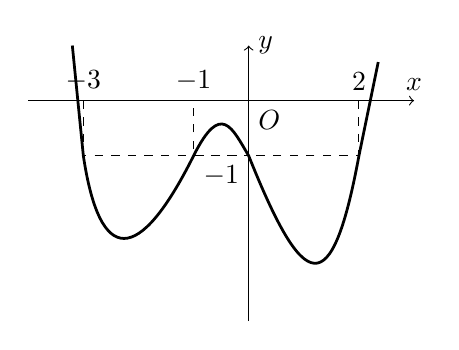
\begin{tikzpicture}[scale=0.7]
            \def\xmin{-4} \def\xmax{3} \def\ymin{-3} \def\ymax{1}
            \draw [->](\xmin,0)--(\xmax,0) node [above]{$x$};
            \draw [->](0,\ymin-1)--(0,\ymax) node [right]{$y$};
            \draw (0,0) node [below right]{$O$};
            \clip (\xmin,\ymin) rectangle (\xmax,\ymax);
            \draw[line width=1pt] (-3.2,1).. controls +(0,0)..(-3,-1)
            .. controls +(0.3,-2) and +(-1,-2)..(-1,-1)
            .. controls +(0.5,1) and +(-0.3,0.5)..(0,-1)
            .. controls +(1,-2.5) and +(-0.5,-2.7)..(2,-1)
            .. controls +(0,0) and +(0,0)..(2.35,0.7)
            ;
            \draw [dashed](-3,0)|-(0,-1) node [below left]{$-1$}-|(-1,0) (2,0)|-(0,-1);
            \foreach \p in {-3,-1,2}
            \draw (\p,0) node [above]{$\p$};
        \end{tikzpicture}
    }
    \loigiai{
        Đặt $x=t^3-2$ ta có $x'=3t^2 \geq 0$ và $t=\sqrt[3]{x+2}$.
        \\
        Khi đó, $y=-2f(x)-2x-1=-2f(t^3-2)-2(t^3-2)-1 \Rightarrow y'=-6t^2f'(t^3-2)-6t^2$.
        \\
        Hàm số $y=-2f(x)-2x-1$ đồng biến thì hàm số $y=-2f(t^3-2)-2(t^3-2)-1$ đồng biến.
        \\
        Ta cần có $-6t^2f'(t^3-2)-6t^2>0 \Leftrightarrow f'(t^3-2)<-1$
        \\
        $\Leftrightarrow \hoac{&-3<t<-1\\&0<t<2} \Leftrightarrow \hoac{&-3<\sqrt[3]{x+2}<-1\\&0<\sqrt[3]{x+2}<2} \Leftrightarrow \hoac{&-29<x<-3\\&-2<x<6.}$
        \\
        Đối chiếu phương án, ta chọn $(-12;-10) \subset (-29;-3)$.
    }
\end{ex}
\begin{ex}%[2D1K1-2]
    Cho hàm số $f(x)$ có bảng xét dấu đạo hàm như hình bên dưới
    \begin{center}
        
\begin{tikzpicture}
            \tkzTabInit[lgt=1.2,espcl=2.5]
            {$x$ /.7, $y'$ /.7}
            {$-\infty$,$-3$,$-1$,$1$,$+\infty$}
            \tkzTabLine{ ,-,$0$,+,$0$,-,$0$, +, }
        \end{tikzpicture}
    \end{center}
    Hàm số $y=f(3-2x)$ đồng biến trên khoảng
    \choice
    {$\left(-\infty;-3\right)$}
    {$\left(2;3\right)$}
    {\True $\left(3;4\right)$}
    {$\left(0;2 \right)$}
    \loigiai{
        Ta có $y'=-2f'(3-2x)$, $y'=0 \Leftrightarrow \hoac{&3-2x=-3\\&3-2x=-1\\&3-2x=1} \Leftrightarrow \hoac{&x=3\\&x=2\\&x=1.}$\\
        Ta có bảng xét dấu
        \begin{center}
            
\begin{tikzpicture}
                \tkzTabInit[lgt=1.2,espcl=3]
                {$x$ /1, $y'$ /1}
                {$-\infty$,$1$,$2$,$3$,$+\infty$}
                \tkzTabLine{ ,-,$0$,+,$0$,-,$0$, +, }
            \end{tikzpicture}
        \end{center}
        Vậy hàm số đồng biến trên khoảng $(3;4)$.
    }
\end{ex}
\begin{ex}%[2D1G1-2]
    \immini{Cho hàm số $y=f(x)$ có đạo hàm liên tục trên $\mathbb{R}$. Đồ thị hàm số $y=f'(3x-1)$ như hình vẽ.
        Hàm số $y=f(x)$ đồng biến trên khoảng nào dưới đây?
        \choice
        {$(-\infty;-6)$}
        {$(1;5)$}
        {$(2;6))$}
        {\True $(-\infty;-7)$}
    }
    {
        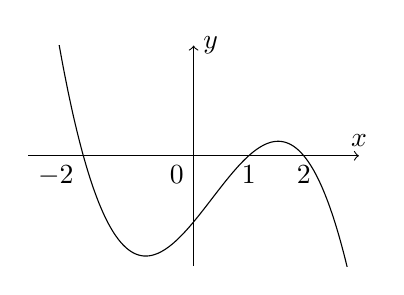
\begin{tikzpicture}[scale=0.7]
            \def\xmin{-3} \def\xmax{3} \def\ymin{-2} \def\ymax{2}
            \draw [->](\xmin,0)--(\xmax,0) node [above]{$x$};
            \draw [->](0,\ymin)--(0,\ymax) node [right]{$y$};
            \draw (0,0) node [below left]{$0$};
            \clip (\xmin,\ymin) rectangle (\xmax,\ymax);
            \draw plot[smooth,samples=100,domain=-4:5] (\x,{-0.3*(\x)^3+0.3*(\x)^2+1.2*\x-1.2});
            \draw (-2,0) node [below left]{$-2$} (1,0) node [below]{$1$} (2,0) node [below]{$2$};
        \end{tikzpicture}
    }
    \loigiai{
        Đặt $x=3t-1$ ta có $g(t)=f(3t-1)\Rightarrow g'(t)=3f'(3t-1)$.
        \\
        $g'(t)>0 \Leftrightarrow f'(3t-1)>0\Leftrightarrow \hoac{&t<-2\\&1<t<2}$.
        \\
        Khi đó $f'(x)<0 \Leftrightarrow \hoac{&\dfrac{x+1}{3}<-2\\&1<\dfrac{x+1}{3}<2} \Leftrightarrow \hoac{&x<-7\\&2<x<5.}$
    }
\end{ex}
\Closesolutionfile{ans}
%\indapan{10}{ans/2D1-1-DEON-2}